\chapter{System Design and Methodology}
\label{chap:methodology}

The primary objective of this thesis is to evaluate the performance impact of Keystone’s enclave isolation mechanisms on representative embedded and systems-level workloads. Specifically, the study aims to quantify the computational overhead introduced by executing applications within a Keystone enclave, compared to their execution in a traditional, non-isolated environment. To this end, a series of controlled experiments were conducted on a virtualized RISC-V platform based on QEMU.

All benchmarks were executed within an emulated environment configured for the RV64GC architecture, which corresponds to the 64-bit RISC-V ISA targeted by Keystone. The QEMU-based emulation provides fine-grained control over system parameters and ensures experimental repeatability by eliminating variability introduced by physical hardware—such as thermal throttling, cache behavior, or platform-specific optimizations. While virtualized, QEMU accurately models instruction execution, privilege-level transitions, memory access patterns, and I/O behavior, making it a viable platform for preliminary performance evaluations of trusted execution environments.

To assess the performance implications of enclave-based isolation, each benchmark was implemented as a standalone enclave application (referred to as an \textit{eapp}), accompanied by a corresponding host application responsible for enclave lifecycle management. The host application, running in user space, handles enclave initialization, benchmark loading, invocation of enclave entry points, and inter-domain communication via edge calls. In contrast, the enclave application is fully isolated by the Keystone runtime and contains only the benchmark logic and associated data structures. This strict separation ensures that the same benchmark codebase can be executed both natively (without isolation) and securely (within an enclave), without requiring structural changes—thus enabling a fair and consistent comparative analysis.

The experimental evaluation was conducted using two well-established benchmarking tools—Dhrystone and CoreMark—each executed under two configurations:

\begin{enumerate}
\item \textbf{Native Execution:} The benchmark runs as a conventional user-space process within the QEMU-emulated Linux system, with no involvement of Keystone's enclave infrastructure.
\item \textbf{Enclave Execution:} The benchmark is loaded into a Keystone enclave, where memory isolation is enforced by the Security Monitor through RISC-V Physical Memory Protection (PMP) mechanisms.
\end{enumerate}

Each benchmark configuration was executed multiple times (typically ten iterations) to mitigate performance variance and ensure statistical robustness. For each run, performance metrics including total execution time, throughput (expressed in DMIPS for Dhrystone and iterations per second for CoreMark), and standard deviation were collected. The analysis focuses on the relative performance degradation incurred in the enclave execution scenario, thereby providing a direct estimate of the overhead associated with enclave-based isolation.

This methodology facilitates a detailed understanding of how Keystone’s architectural design and isolation primitives influence runtime performance. The controlled and repeatable test environment, combined with standardized benchmarking tools and consistent measurement practices, ensures that the results are both reliable and meaningful. Ultimately, the findings offer valuable insights into the trade-offs between security and efficiency in open-source TEE frameworks and inform future efforts in trusted system design.

\section{Experimental Platform and Environment}
\label{sec:experimental-setup}

The experimental setup was designed to enable reliable, repeatable evaluation of the Keystone Trusted Execution Environment (TEE) without requiring physical RISC-V hardware. To achieve this, a virtualized testbed was constructed using a RISC-V-specific fork of the QEMU emulator running on an Ubuntu 22.04 LTS host system. This emulated environment provides fine-grained control over system configuration, facilitating flexible testing of Keystone enclaves while accurately modeling a real RISC-V platform.

QEMU, an open-source hardware emulator, was configured to emulate the RV64GC (64-bit general-purpose) RISC-V architecture, fully compatible with Keystone’s software stack. This choice reflects Keystone’s target deployment on modern RISC-V platforms and allows access to enclave memory protection and privilege separation features managed by the Keystone Security Monitor. Ubuntu 22.04 LTS was selected for its long-term support, stability, and compatibility with the Keystone development toolchain, serving as a robust platform for building all components including the QEMU binary, Keystone kernel driver, runtime, and benchmark binaries.

The build process utilizes a combination of \texttt{Make} and Buildroot. Buildroot generates the embedded Linux root filesystem, cross-compiles necessary system libraries, and configures the Linux kernel running inside the QEMU guest. The Make-based system orchestrates compilation and deployment of Keystone components such as the runtime, Security Monitor, and kernel modules, ensuring reproducible builds targeting the QEMU RV64 environment.\footnote{Key configuration parameters include the QEMU platform, RV64 CPU architecture, and Buildroot settings optimized for Keystone enclave support.} 

Launching the virtualized system is managed through a Makefile-driven workflow defined in the \texttt{run.mk} file, which encapsulates QEMU configuration and execution commands. Several runtime parameters are exposed as Makefile variables for flexibility, including:

\begin{itemize}
    \item \texttt{QEMU\_PORT} (default: 9821) — SSH port forwarding to access the QEMU guest.  
    \item \texttt{QEMU\_DBG\_PORT} (default: \texttt{QEMU\_PORT} + 1) — TCP port for GDB debugging.  
    \item \texttt{QEMU\_RAM\_SIZE} (default: 128M) — amount of emulated RAM.  
    \item \texttt{QEMU\_CORE\_COUNT} (default: 2) — number of virtual CPU cores.
\end{itemize}

QEMU is launched with flags specifying the machine type (\texttt{virt}), boot ROM and firmware, kernel and root filesystem images, VirtIO devices for block storage and networking, and network forwarding for SSH access. Optionally, a cache plugin \cite{mandour2021cache} can be enabled to provide detailed logging of cache events such as hits, misses, and evictions. This plugin offers deeper insight into the memory hierarchy’s behavior during enclave execution, aiding analysis of performance impacts due to cache and memory isolation overhead.

The cache plugin \cite{mandour2021cache} parameters are fully configurable at runtime, including:

\begin{itemize}
    \item Instruction cache: \texttt{icachesize}, \texttt{iblksize}, \texttt{iassoc} — size, block size, and associativity.  
    \item Data cache: \texttt{dcachesize}, \texttt{dblksize}, \texttt{dassoc} — analogous data cache parameters.  
    \item Eviction policy: \texttt{evict=lru|rand|fifo}.  
    \item Logging limits: \texttt{limit=TOP\_N} for number of top thrashing instructions to record.  
    \item Number of cores monitored: \texttt{cores=N\_CORES}.
\end{itemize}

For example, to configure the cache plugin with 8 KB L1 instruction and data caches, 64-byte blocks, 4-way associativity, 2 cores, and LRU eviction, the following command is used:

\begin{lstlisting}
make QEMU_PLUGIN_ARGS="dcachesize=8192,dassoc=4,dblksize=64, \
icachesize=8192,iassoc=4,iblksize=64,cores=2,evict=lru" run
\end{lstlisting}

While the plugin logs comprehensive cache activity, it cannot isolate cache events exclusively caused by enclave operations. Therefore, cache data interpretation requires caution when attributing performance effects specifically to enclaves.

Debugging support is available by enabling the \texttt{KEYSTONE\_DEBUG} flag, which starts QEMU’s built-in GDB server and halts execution at startup for remote debugging. After booting the QEMU guest, the Keystone kernel driver is loaded manually using:

\begin{lstlisting}
modprobe keystone-driver
\end{lstlisting}

This step initializes enclave functionality, allowing benchmark binaries to be securely loaded and executed within isolated memory regions managed by the Security Monitor.

Additional Makefile targets enable remote command execution over SSH and connection to the RISC-V GDB debugger for low-level inspection of enclave state. Debugging requires recompiling Keystone with debugging enabled, typically invoked as:

\begin{lstlisting}
KEYSTONE_DEBUG=y make run
make debug-connect
\end{lstlisting}

QEMU’s built-in GDB server provides visibility into registers, memory, and exceptions, aiding low-level inspection and troubleshooting of enclave operations.

Overall, this integrated virtualized environment and build system provide a flexible, controlled platform for detailed evaluation of Keystone’s performance and security properties. The modular Makefile-driven workflow streamlines configuration, deployment, and debugging, enabling efficient development and benchmarking without dependence on physical hardware. %Further technical details on build dependencies and configuration options are documented in the \textbf{Appendix}.

\section{Integration of Kyber into Keystone}
\label{sec:kyber-enclave}

To comprehensively evaluate the performance characteristics of cryptographic workloads within a trusted execution environment, this study incorporates the Kyber key encapsulation mechanism (KEM), a lattice-based post-quantum cryptographic primitive. Kyber has garnered significant attention as a leading candidate in the NIST post-quantum cryptography standardization process, offering a robust balance of security, performance, and suitability for deployment on resource-constrained devices. Its integration within a secure enclave environment highlights the practical implications of deploying advanced cryptographic primitives where hardware-based isolation is critical for protecting sensitive operations and data.

The Kyber implementation employed in this work is derived from a well-maintained, lightweight C reference library, chosen for its portability and compatibility with embedded systems. This implementation was integrated into the Keystone enclave framework with minimal modification to preserve fidelity to the original cryptographic routines and avoid introducing artifacts that might bias performance measurement. Both the IND-CPA (indistinguishability under chosen-plaintext attack) and IND-CCA (indistinguishability under chosen-ciphertext attack) variants of Kyber were considered, with the primary cryptographic operations — key generation, encapsulation, and decapsulation — being individually invoked inside the enclave to facilitate granular performance profiling.

The following critical Kyber functions were separately instrumented and timed to capture their distinct computational demands:

\begin{itemize}
    \item \texttt{indcpa\_keypair} — Key pair generation for the IND-CPA variant.
    \item \texttt{indcpa\_enc} — Encryption (encapsulation) under IND-CPA assumptions.
    \item \texttt{indcpa\_dec} — Decryption (decapsulation) under IND-CPA assumptions.
    \item \texttt{kyber\_keypair} — Enhanced key pair generation supporting IND-CCA.
    \item \texttt{kyber\_encaps} — IND-CCA-compliant encapsulation.
    \item \texttt{kyber\_decaps} — IND-CCA-compliant decapsulation.
\end{itemize}

Each of these operations was executed across the five representative system configurations defined in Section~\ref{sec:param-variation}, which span a broad range of memory capacities, core counts, and execution modes. To ensure measurement accuracy and reduce variability from transient system states, ten iterations were run per configuration with the first iteration discarded as a warm-up phase. Execution timing was obtained using the enclave’s internal high-resolution timer API, capturing secure-world runtime exclusively. In parallel, external system-level metrics — such as CPU usage, memory footprint, and context switching counts — were gathered from the host environment to provide contextual insights into system overhead and resource utilization.

Unlike the synthetic benchmarks Dhrystone and CoreMark, Kyber’s workload is characterized by its intensive use of polynomial arithmetic, noise sampling, and number-theoretic transform (NTT) operations, all of which impose a distinct computational profile. Notably, Kyber exhibits a predominantly CPU-bound execution pattern, with relatively limited memory demands. This profile contrasts with cache- and memory-intensive workloads, which often demonstrate sensitivity to cache size, associativity, and eviction policies. Additionally, Kyber’s current implementation executes sequentially without exploiting parallelism or multithreading, making it well-suited for analysis within single-threaded enclave contexts.

It is important to note that the QEMU cache modeling plugin \cite{mandour2021cache} utilized for this study provides comprehensive logging of cache events and misses across the entire emulated system rather than isolating activity specific to the enclave or Kyber operations. Consequently, while cache plugin data enriches understanding of system-wide memory behavior, it does not enable direct attribution of cache hits or misses exclusively to Kyber’s execution. This limitation underscores the challenges of fine-grained performance attribution within complex emulation environments but does not diminish the value of combined timing and system-level metrics in capturing overall workload behavior.

Collectively, the measurement approach — leveraging both enclave-internal timers and host-level monitoring — facilitates a nuanced characterization of Kyber’s execution within a trusted environment. This methodology reveals how cryptographic routines with intricate arithmetic and memory access patterns perform under enclave constraints, including the overhead introduced by secure isolation and the impact of varying system resources such as memory size and CPU core availability.

Kyber’s inclusion in the benchmark suite extends the evaluation beyond traditional CPU-bound synthetic workloads, providing a practical example of a security-critical, compute-heavy application with significant implications for post-quantum readiness in embedded and secure computing contexts. The insights derived from profiling Kyber within Keystone enclaves inform considerations around enclave design, resource allocation, and the feasibility of deploying advanced cryptographic primitives in isolated environments with minimal performance degradation.

Kyber serves as a representative case study for secure, non-parallelizable cryptographic workloads executed within enclave boundaries. Its performance characteristics complement those observed in more generic benchmarks by illuminating the interplay between cryptographic computation, enclave isolation overhead, and system resource scaling. This comprehensive evaluation underpins recommendations for enclave provisioning and optimization in future secure computing platforms.


\section{Benchmarking Suite and Metrics}
\label{sec:benchmarking-tools}

To evaluate the performance impact of the Keystone Trusted Execution Environment (TEE) comprehensively, this study employs two well-established synthetic benchmarks: \textit{Dhrystone} and \textit{CoreMark}. Both are widely used in the embedded systems community and are well-supported in the RISC-V ecosystem, making them natural choices to assess Keystone’s behavior in secure versus non-secure execution modes. These benchmarks capture a broad spectrum of processor activities relevant to enclave execution—such as integer arithmetic, control flow, and memory access patterns.

The Dhrystone benchmark~\cite{weiss2002dhrystone} has been used for decades to measure general-purpose processor performance, especially in scenarios where floating-point operations and file I/O are not critical. Its focus on integer calculations and control structures—such as loops, function calls, and basic data handling—is representative of many embedded and real-time applications. Thanks to its simplicity and minimal memory usage, Dhrystone~\cite{weiss2002dhrystone} provides a clean baseline measure of raw processor capability. For this study, the RISC-V implementation of Dhrystone was obtained from the official \texttt{riscv-tests} repository to ensure accurate execution on the target platform. The benchmark was executed twice under identical conditions—once in native, non-secure mode and once inside a Keystone enclave. This dual setup facilitates precise measurement of the performance overhead imposed by Keystone’s security mechanisms, including memory isolation and context-switching between secure and non-secure worlds.

Dhrystone results are typically reported as "Dhrystones per second," quantifying how many benchmark iterations complete in one second. For broader comparability across different processor architectures, these results are normalized to Dhrystone MIPS (DMIPS), which estimates the effective instruction throughput in millions of instructions per second. This normalization allows meaningful performance comparisons by smoothing out architectural differences. In this study, comparing DMIPS between enclave and native executions highlights the raw performance impact of enabling the TEE.

To complement Dhrystone and gain insight into more complex system behavior, the CoreMark benchmark~\cite{gal2012exploring} was also employed. Developed by the Embedded Microprocessor Benchmark Consortium (EEMBC), CoreMark~\cite{gal2012exploring} addresses some limitations of Dhrystone by incorporating workloads that are closer to real-world embedded applications. It includes linked list manipulations, matrix operations, and finite state machine processing—tasks common in embedded software. Although still CPU-centric, CoreMark~\cite{gal2012exploring} exercises the memory subsystem more heavily through dynamic data structures, thereby exposing performance effects related to cache usage and memory protection features within a TEE.

The CoreMark version used in this study was sourced from the SiFive repository on GitHub\footnote{\url{https://github.com/sifive/benchmark-coremark}, accessed August 2025}, providing a RISC-V-optimized build compatible with Keystone. Like Dhrystone, CoreMark was run in both native and enclave modes, with results reported as "Iterations Per Second" (IPS), indicating how many complete benchmark runs occur per second. Because CoreMark combines arithmetic and memory operations, IPS delivers a more comprehensive view of system performance, reflecting both CPU and memory subsystem efficiency.

In addition to primary performance metrics—DMIPS for Dhrystone and IPS for CoreMark—this study also analyzed supporting metrics to better characterize system behavior. Overall execution time, measured in wall-clock seconds, was recorded for each benchmark run. Comparing execution times between enclave and native modes quantifies latency introduced by secure execution, including overheads from memory protection, context switching, and enclave isolation mechanisms.

Variability across runs was assessed through the standard deviation of benchmark results over multiple iterations. A low standard deviation signifies consistent and reliable performance, whereas higher variability might indicate sensitivity to system noise, scheduling delays, or other environmental factors.

Both Dhrystone~\cite{weiss2002dhrystone} and CoreMark~\cite{gal2012exploring} are CPU-intensive benchmarks, making them particularly useful for this study’s focus on processor and memory subsystem behavior under secure execution. Dhrystone targets raw integer and control flow performance, offering a clear view of base processor throughput, while CoreMark’s more sophisticated workload reveals broader impacts of the TEE’s security mechanisms, especially regarding memory interactions. Neither benchmark involves file I/O or persistent storage; therefore, this study does not assess storage-related TEE features such as secure disk access or file encryption, which would require alternative benchmarking approaches.

By combining these two benchmarks with detailed timing and variability analysis, this study provides a well-rounded and nuanced understanding of the trade-offs involved in securing execution via Keystone enclaves on RISC-V platforms.

\section{Parameter Configuration and Variation}
\label{sec:param-variation}

To rigorously assess how architectural and system-level parameters influence the performance of workloads executed within secure enclaves, this study undertook a systematic exploration of configurable runtime characteristics on the simulated RISC-V platform. Specifically, we varied four principal dimensions: physical memory size, the number of processor cores, execution mode (sequential versus parallel), and cache configuration. These parameters were chosen based on their known relevance to workload performance and enclave behavior, and were adjusted within the bounds of what is supported by the QEMU-based virtual platform and the Keystone framework.

The overarching objective of this variation was to uncover the extent to which system-level constraints and resource allocations impact both trusted (enclave) and non-trusted (native) execution. By exploring diverse configurations, we aimed to characterize how resource limitations (e.g., constrained memory or limited cores) manifest in performance degradation, and to what degree secure execution amplifies or mitigates these effects.

To simulate cache behavior, we employed the QEMU TCG plugin framework, specifically leveraging the cache modeling capabilities introduced by Mandour et al. \cite{mandour2021cache}. This plugin facilitates the modeling of per-core instruction and data caches and enables the collection of aggregate system-wide cache statistics. While it does not provide cycle-accurate timing nor isolate enclave-specific cache behavior, its ability to log cache access and miss patterns uniformly across all benchmark executions proved sufficient for analyzing cache-related effects in both secure and non-secure modes. The insights gleaned from this analysis, though approximate, were instrumental in identifying general cache utilization trends under various workloads and resource configurations.

Given the expansive parameter space created by the combination of memory size, core count, execution mode, and cache settings, it was neither practical nor necessary to exhaustively benchmark every possible configuration. Instead, we curated a set of five representative system configurations that collectively span a meaningful range of the performance spectrum—from minimal, resource-constrained environments to well-provisioned, multicore systems operating at near full capacity. These configurations are detailed in Table~\ref{tab:configurations}.

\begin{table}[h]
\centering
\begin{tabular}{|l|c|c|c|p{7.5cm}|}
\hline
\textbf{Config Name} & \textbf{RAM} & \textbf{Cores} & \textbf{Execution} & \textbf{Rationale} \\
\hline
Low-End Baseline     & 64M         & 1             & Sequential         & Serves as a minimal configuration, enabling the establishment of baseline performance under constrained conditions. Useful for measuring the raw impact of enclave mechanisms in resource-starved environments. \\
\hline
Balanced Parallel    & 128M        & 2             & Parallel           & Captures early-stage scaling behavior with modest multicore setups. Helps isolate the overhead introduced by enclave entry/exit in light parallel workloads. \\
\hline
Mid-Range Sequential & 256M        & 4             & Sequential         & Provides a view into how increasing core count and memory capacity affect performance in the absence of thread-level parallelism. Useful for understanding system scalability independent of synchronization effects. \\
\hline
High-End Parallel    & 512M        & 6             & Parallel           & Represents a robust configuration where memory and cores are sufficiently provisioned. Designed to observe near-ideal parallel execution and potential scalability limits of the enclave framework. \\
\hline
Max Capacity Stress  & 2G          & 10            & Parallel           & Pushes the simulated platform to its upper bounds. Intended to explore saturation points, resource contention, and diminishing returns under heavy system load. \\
\hline
\end{tabular}
\caption{Summary of representative configurations used in performance evaluation.}
\label{tab:configurations}
\end{table}

In preliminary testing, a number of alternative configurations were explored to validate the diversity and coverage of the selected set. These included scenarios such as single-core systems with excessively large memory allocations and many-core setups with highly constrained memory. However, these combinations typically resulted in either underutilized resources or pathological behavior (e.g., excessive paging or context switching), without contributing new insight beyond what was captured by the five chosen profiles. For example, increasing memory size on a single-core system had negligible impact due to CPU-bound bottlenecks, while increasing core counts in systems with limited memory often led to high levels of involuntary context switching and scheduling overhead.

In addition to varying core and memory resources, three distinct cache configurations were tested across all system profiles to assess the sensitivity of enclave and native workloads to cache architecture. These configurations included:

\begin{itemize}
    \item A baseline setup featuring 8\,KB, 4-way set-associative caches with an LRU replacement policy
    \item An enlarged cache with 32\,KB size and 8-way associativity, reflecting more generous cache resources
    \item A fixed-size cache using FIFO and random eviction policies to model alternative eviction behaviors
\end{itemize}

All configurations used a consistent block size of 64 bytes to preserve spatial locality across workloads. Although the cache modeling plugin captures system-wide statistics and does not differentiate between enclave and non-enclave activity, observed trends—such as shifts in cache miss rates and access patterns—were analyzed in conjunction with benchmark-level behavior to infer their contribution to observed performance variations.

To enable direct and consistent comparisons, each benchmark was executed in both native and enclave modes under every configuration. This mirrored design allowed for clear isolation of the performance penalties introduced by enclave execution and helped disentangle architectural effects from security-related overhead.

\section{Data Collection and Reproducibility}
\label{sec:data-collection}

To ensure the integrity, consistency, and scientific validity of the performance evaluation, all benchmark experiments were conducted within a tightly controlled and reproducible virtualized environment. The entire measurement campaign was executed on a simulated RISC-V platform using the QEMU emulator, which served as the foundation for both native and enclave-based workloads. This consistent virtualization layer eliminated hardware variability and allowed for precise control over system resources such as memory, core count, and cache characteristics.

Each system configuration, as defined in Section~\ref{sec:param-variation}, was evaluated using the Dhrystone, CoreMark, and Kyber benchmarks. For each benchmark, tests were run in both native (non-enclave) and enclave execution modes to facilitate direct comparative analysis of performance overheads introduced by trusted execution.

To reduce transient measurement noise and improve the robustness of collected data, each benchmark experiment was repeated ten times per configuration. The first execution was discarded in all cases to account for initialization artifacts such as dynamic binary translation warm-up and memory allocation caching within the QEMU runtime. The remaining nine runs were averaged to produce stable and representative performance figures. In addition to computing the arithmetic mean, the standard deviation was recorded to provide a measure of variability across runs.

The primary performance metric collected was **total wall-clock execution time**, as measured from within the guest Linux environment using high-resolution timers (e.g., \texttt{clock\_gettime()}) or the Keystone timer API in enclave mode. For Dhrystone and CoreMark, benchmark-specific throughput metrics were also recorded, including Dhrystone MIPS (DMIPS) and iterations per second. These allowed for workload-specific efficiency comparisons across configurations.

In addition to these high-level metrics, detailed system-level runtime statistics were gathered using standard Linux facilities such as the \texttt{/proc} filesystem and the \texttt{getrusage()} system call. These included:

\begin{itemize}
    \item \textbf{User and system CPU time:} Total time spent in user-space and kernel-space respectively.
    \item \textbf{Maximum resident set size (RSS):} Peak memory consumption during execution.
    \item \textbf{Page fault statistics:} Number of minor (soft) and major (hard) page faults incurred during the benchmark.
    \item \textbf{Context switching behavior:} Number of voluntary and involuntary context switches, indicating scheduling and synchronization overhead.
\end{itemize}

These runtime indicators were critical in diagnosing performance behaviors that could not be attributed to CPU throughput alone. For instance, elevated context switch counts in parallel configurations were often correlated with increased enclave transition overhead or CPU oversubscription, especially in memory-constrained environments.

Cache-related metrics were obtained using the QEMU TCG plugin cache model described earlier. This plugin logs all instruction and data cache accesses and cache misses at the system level. While the plugin lacks enclave-specific visibility and does not model hardware-specific cache timing, it provides a consistent and useful proxy for analyzing trends in memory access behavior. Cache metrics were aligned with benchmark execution phases to identify correlations between cache activity and observed performance shifts.

To compute the enclave-specific performance overhead, we employed a normalized overhead metric defined as the relative increase in execution time between enclave and native modes:

\[
\text{Overhead (\%)} = \left( \frac{\text{Enclave Time} - \text{Native Time}}{\text{Native Time}} \right) \times 100
\]

This percentage-based formulation allows for direct cross-comparison of overheads across workloads with differing baseline durations. It also facilitates trend identification across system configurations, particularly when assessing scaling behaviors.

For reproducibility, all benchmarking scripts, system configurations, QEMU command-line options, Keystone runtime parameters, and cache plugin settings were version-controlled using Git. Raw benchmark outputs, kernel logs, and cache plugin trace files were archived and documented. A complete snapshot of the experimental infrastructure, along with scripts to regenerate results, is provided in Appendix~\ref{appendix:cache-plugin}. This archival effort ensures that all reported results can be independently verified and reproduced by future researchers or evaluators.

\begin{figure}[H]
\centering
\begin{tikzpicture}[node distance=1.75cm]
\node (start)   [process] {Start: Define Benchmark Set};
\node (config)  [process, below of=start] {Select Hardware Configuration};
\node (native)  [process, below of=config] {Run Benchmarks in Native Mode};
\node (enclave) [process, below of=native] {Run Benchmarks in Enclave Mode};
\node (metrics) [process, below of=enclave] {Collect Performance Metrics};
\node (analyze) [process, below of=metrics] {Compare and Analyze Overheads};
\node (end)     [process, below of=analyze] {Store Logs and Archive Results};

\draw [arrow] (start)   -- (config);
\draw [arrow] (config)  -- (native);
\draw [arrow] (native)  -- (enclave);
\draw [arrow] (enclave) -- (metrics);
\draw [arrow] (metrics) -- (analyze);
\draw [arrow] (analyze) -- (end);
\end{tikzpicture}
\caption{Benchmarking and Data Collection Workflow}
\label{fig:benchmarking-workflow}
\end{figure}

\begin{figure}[H]
\centering
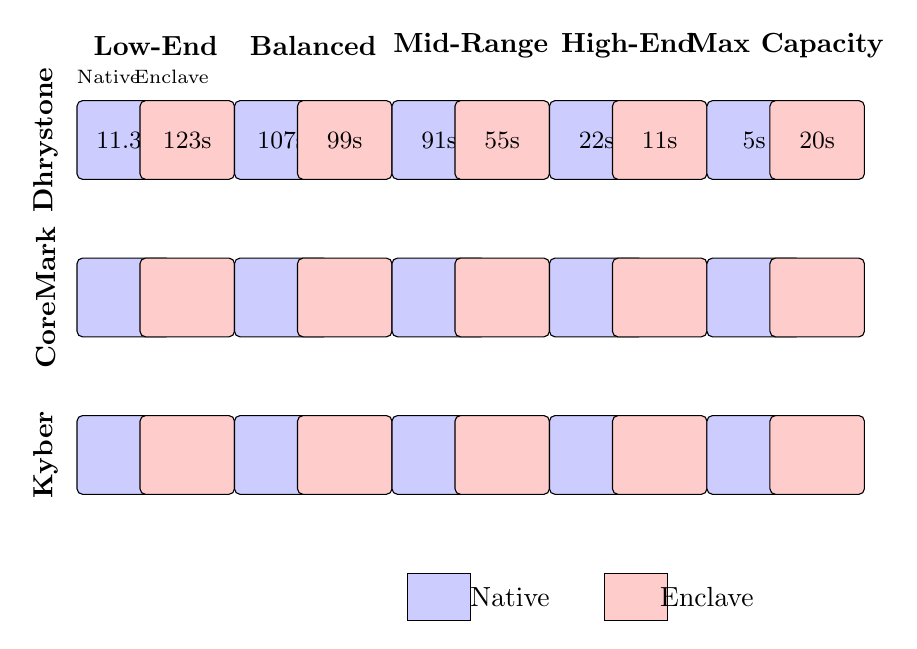
\begin{tikzpicture}[
    native/.style={draw, fill=blue!20, minimum width=1.2cm, minimum height=1cm, font=\small, rounded corners=2pt},
    enclave/.style={draw, fill=red!20, minimum width=1.2cm, minimum height=1cm, font=\small, rounded corners=2pt},
    label/.style={font=\bfseries, align=center},
    cell/.style={draw, minimum width=1cm, minimum height=0.6cm},
    every node/.style={inner sep=2pt}
]

% Column labels
\node[label] at (2.4, 6.2) {Low-End};
\node[label] at (4.4, 6.2) {Balanced};
\node[label] at (6.4, 6.2) {Mid-Range};
\node[label] at (8.4, 6.2) {High-End};
\node[label] at (10.4, 6.2) {Max Capacity};

% Row labels
\node[label, rotate=90] at (1, 5) {Dhrystone};
\node[label, rotate=90] at (1, 3) {CoreMark};
\node[label, rotate=90] at (1, 1) {Kyber};

% Dhrystone row
\node[native] at (2, 5) {11.3s};
\node[enclave] at (2.8, 5) {123s};

\node[native] at (4, 5) {107s};
\node[enclave] at (4.8, 5) {99s};

\node[native] at (6, 5) {91s};
\node[enclave] at (6.8, 5) {55s};

\node[native] at (8, 5) {22s};
\node[enclave] at (8.8, 5) {11s};

\node[native] at (10, 5) {5s};
\node[enclave] at (10.8, 5) {20s};

% CoreMark row (empty placeholders for now)
\foreach \x in {2,4,6,8,10} {
    \node[native] at (\x, 3) {};
    \node[enclave] at (\x+0.8, 3) {};
}

% Kyber row (empty)
\foreach \x in {2,4,6,8,10} {
    \node[native] at (\x, 1) {};
    \node[enclave] at (\x+0.8, 1) {};
}

% Native / Enclave labels inside or above boxes if needed
\node[font=\scriptsize] at (1.8, 5.8) {Native};
\node[font=\scriptsize] at (2.6, 5.8) {Enclave};

% Legend
\node[draw, fill=blue!20, minimum width=0.8cm, minimum height=0.6cm] at (6, -0.8) {};
\node at (6.9, -0.8) {Native};

\node[draw, fill=red!20, minimum width=0.8cm, minimum height=0.6cm] at (8.5, -0.8) {};
\node at (9.4, -0.8) {Enclave};

\end{tikzpicture}
\caption{Experiment Matrix: Benchmarks Across Configurations and Execution Modes}
\label{fig:experiment-matrix}
\end{figure}
